%********************************************************************************************
%								COMANDOS ÚTILES PARA LATEX EN ESTE TP							
%
%	\ : espacio simple
%	\\ : nueva línea
%	\par : va a la línea de abajo y deja sangría
%	\vspace{##tamaño en pt##} o \vspace{\baselineskip} en general:
%								 para dejar un espacio vertical
%	\textbf{text} :text en negrita
%	\textit{text} :text en itálica
%
% GRAFICOS CENTRADOS:
%	\begin{center}
%		\includegraphics[width=\textwidth]{./img/##ruta imagen (no hace falta extension)##}
%	\end{center}
%		--> se pueden agregar atributos como scale por si se hace muy grande
%
% TABLAS CENTRADAS:
%	\begin{center}
%	\begin{tabular}{|c|c|}
%	\hline
%	\ \textbf{Programa} & \textbf{Ticks} \\
%	\hline
%		ASM & 675127609 \\
%	\hline
%	\end{tabular}
%	\end{center}
%
% ALGORITMOS (EN VARIOS LENGUAJES):
% \begin{lstlisting}
%	void sumoDiez(int &num)
%	{
%	    num += 10;
%	}
%	
%	int main()
%	{
% 	   int i;
%	    int numeroAProcesar = 20;
%	    for (i = 0; i < 50; i++)
%	    {
%	        sumoDiez(numeroAProcesar);	//Proceso el numero en cada ciclo
%	    } 
%	    return 0;
%	}
%	\end{lstlisting}
%
% para info sobre todo lo que tiene el package detallado:
% http://en.wikibooks.org/wiki/LaTeX/Source\_Code\_Listings
%
%********************************************************************************************

\documentclass[10pt,a4paper]{article}
\usepackage[utf8]{inputenc} % para poder usar tildes en archivos UTF-8
\usepackage[spanish]{babel} % para que comandos como \today den el resultado en castellano
\usepackage{a4wide} % márgenes un poco más anchos que lo usual
%\usepackage{geometry}

%\usepackage{layout}

%\geometry{
%  includeheadfoot,
%  margin=2.7cm
%}

\usepackage[conEntregas]{caratula}
\usepackage{amssymb}
\usepackage{fancybox}
\usepackage[usenames,dvipsnames]{color}
\usepackage{hyperref}
\usepackage{listings}
\usepackage{clrscode3e}
\usepackage{xcolor}
\usepackage{amsmath}


\hypersetup{
    colorlinks,
    citecolor=black,
    filecolor=black,
    linkcolor=black,
    urlcolor=black
}

\lstdefinestyle{customc}{
  belowcaptionskip=1\baselineskip,
  breaklines=true,
  frame=L,
  xleftmargin=\parindent,
  language=C,
  showstringspaces=false,
  basicstyle=\footnotesize\ttfamily,
  keywordstyle=\bfseries\color{green!40!black},
  commentstyle=\itshape\color{purple!40!black},
  identifierstyle=\color{blue},
  stringstyle=\color{orange},
}

\lstset{escapechar=@,style=customc}

\begin{document}

\titulo{Trabajo Práctico 2}
\subtitulo{Develando la mentira de los megapíxeles [Primera entrega]}

\fecha{\today}

\materia{Métodos Numéricos}
\grupo{Grupo Autodenominado "Los Pichis"}

\integrante{De Sousa Bispo, Germán Edgardo}{359/12}{german\_nba11@hotmail.com}
\integrante{De Sousa Bispo, Mariano Edgardo}{389/08}{marian\_sabianaa@hotmail.com}
\integrante{Valdés Castro, Tobías}{800/12}{tobias.vc@hotmail.com}


\maketitle

\tableofcontents
\newpage

\section*{Introducción}
\addcontentsline{toc}{section}{Introducción}

Luego de haber llevado a cabo el TP1 y el TP2 de métodos númericos, la excelente compañía \textbf{Adobby} se vio interesada en nosotros. En vista de que se presentaron tres puestos libres en la compañia (se dice que tres de sus empleados, un flaquito de anteojos, un colorado y una sabelotodo, partieron en búsqueda de un nuevo trabajo en ``El Que No Debe Ser Nombrado''), los recruiters de la empresa lanzaron un desafío para encontrar los reemplazantes de lo que llamaban ``el trío mágico'', y suplantarlos de esta manera en sus puestos de \textit{Ninja Gurú Jedi Master: The image demosaicing god.}

\par 
El desafío consiste en diseñar, implementar y analizar un algoritmo para resolver el
problema de demosaicing. El mismo consiste en obtener una imagen con información en los 3 canales (colores rojo, verde y azul) para cada pixel, a partir de la información capturada por un sensor de una cámara digital marca \textit{``Fotos Casi en Movimiento''}. Para esto se asume que la información captada por el sensor es
correcta y se trata de inferir los valores de los dos canales faltantes en cada uno de los píxeles de la imagen.
\par 
Con el fin de no tener que invocar artes oscuras para resolver este problema, el desafío plantea trabajar solo sobre el Bayer Array. El mismo consiste en alternar filas de rojo y verde o verde y azul. Cada color no recibe una fracción igual en el area ya que el ojo humano es mas sensitivo a la ``luz verde''. Este tipo de arreglo tiene el doble de elementos verdes que rojos o azules, lo cual produce una imagen que aparenta tener menos ruido y mayor detalle que si se trataran los tres colores por igual. El motivo por el que sucede esto escapa los efectos de este trabajo práctico.
\par 
Como parte del desafío de lo que denominaron \textit{``El torneo de los Tres Programadores''}, \textit{Adobby} pidió que se implementaran varios métodos para poder recrear la imagen a partir de lo que tomó la cámara.


\section{Desarrollo}

\subsection{Implementación}

Antes de poder empezar a trabajar se necesita una imagen obtenida por alguna cámara de fotos digital, pero antes de poder observarla en el visor. Esto es, \textit{que no tenga hecho el proceso de demosaicing}, ya que es justamente esto lo que se plantea resolver en el trabajo práctico. Por simpleza, la obtención del archivo con la representación en forma de mosaico se hace a partir de una imagen normal (con el proceso de \textit{mosaicing}) y no de lo que capten los sensores de una cámara. El algoritmo que se ocupa de este proceso fue realizado en \textit{Matlab} y pasa entonces una imagen normal a una imagen con un mosaico que sigue los lineamientos del Bayer Array propuesto (el más utilizado hoy en día).

Igualmente, no utilizamos una librería/biblioteca\footnote{Son libres de elegir la palabra que quieran sin juzgar, se los prometemos.} de C++ que se ocupe de cargar imágenes, por lo tanto después de procesar una imagen normal con el algoritmo de \textit{mosaicing}, también se la lleva desde \textit{Matlab} a un archivo de texto que la represente. Este archivo tiene alto y ancho de la imagen y los valores de la matriz que la conforman en escala de grises (es decir, pasamos las 3 capas de colores a una sola capa ya que no hay canales que se superpongan en este tipo de imágenes con anteriores al \textit{demosaicing}). Además, como ya sabemos donde se encuentra cada color del Bayer Array, podemos cargar la imagen con nuestro código en C++ sin mayores problemas.

Nuestro programa recibe luego como parámetros el nombre de algún archivo que contenga la información antes explicada que represente a una imagen con el proceso de \textit{mosacing}. Además, otro parámetro que se le pasa a nuestro programa es el del tipo de filtro a aplicar. En caso del algoritmo de Malvar, He y Cutler, también se obtiene un tercer parámetro \textbf{$\alpha$} que caracteriza este filtro en particular.

Acercándonos un poco más al código, lo primero que se hace es tomar el archivo obtenido por parámetro y, a partir de sus datos, crear la \textit{bayerImage} correspondiente, que luego es utilizada para aplicar el filtro que elegimos mediante el segundo parámetro.

Finalmente, luego de la ejecución del filtro elegido, se guardan tres archivos correspondientes a las capas verde, azul y roja de la imagen obtenida. Estos archivos tienen un formato que permite ser leído por \textit{Matlab}, desde donde posteriormente se van a recrear las imágenes.

A su vez, los algoritmos de cálculo de calidad cuantitativa también serán aplicados \textit{Matlab}, ya que se nos hace mucho más fácil programarlos allí con las facilidades que nos ofrece el \textit{toolbox} de edición de imágenes. Las calidades medidas en nuestro TP son PSNR\footnote{\textit{Peak Signal to Noise Ratio}} y SSIM\footnote{\textit{Structural SIMilarity}} y se encuentran en el paquete de \textit{Matlab R2014a}, pero ya que no lo tenemos programamos PSNR e hicimos uso de un SSIM ya existente [3]. Todos estos scripts de \textit{Matlab} se pueden encontrar en la carpeta \textit{matlab}.

\vspace{2\baselineskip}

Todas la implementaciones que se mostrarán a continuación, se hicieron bajo la base de obtener el siguiente bayer array:

	\par 
	\begin{center}
		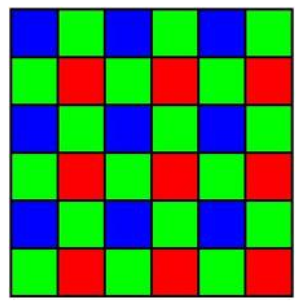
\includegraphics[scale=0.4]{./img/bayerarray.png}
		\par 
		\footnotesize\textit{Modelo de Bayer Array utilizado.}
	\end{center}
	\par 
	
Como podemos notar, e indexando las filas y columnas desde 0, los píxeles azules se encuentran en las posiciones de fila par y columna par. Por otro lado, el color rojo aparece en las filas impares y columnas impares, mientras que el color verde se encuentra en toda posición que no cumple la misma paridad entre columnas y filas.
\par 
Una vez dicho esto, comenzamos con el análisis de las implementaciones realizadas para los siguientes filtros.
	
\subsubsection{Closest Neighbor}

Este filtro se basa en rellenar los valores faltantes copiando al vecino más
cercano del pixel, siempre y cuando tenga una observación real en el mismo canal que se está tratando averiguar. Este fundamento se basa en considerar que el valor de dos pixeles cercanos no debe variar mucho respecto de un mismo canal. De esta manera, podemos obtener toda la información que necesitamos a partir de contemplar el entorno de cada pixel.
\par 
En nuestro caso, se decidió dividir los casos dependiendo si la información que buscamos corresponde al canal verde o a otro canal.
\par 
Como ya se explicó previamente, el color verde va a ser encontrado en las columnas impares y filas pares al igual que en las columnas pares y filas impares. De esta manera, y mirando el modelo de bayer array que se planteó previamente, decidimos tomar los valores que se encuentra en la fila superior y misma columna, y los valores en la columna anterior y misma fila (es decir, tomar el valor del pixel justo encima y el que se encuentra justo a la izquierda). Sin embargo, a qué canal corresponde cada valor depende de en qué fila se encuentre el pixel que quiero reconstruir. Es por esto que se hace un chequeo sobre la fila del píxel.
\par 
Solo a manera ilustrativa e informativa, se muestra en qué sector del código se realiza esto (método \textit{FilterImage()}): 
\begin{lstlisting}
if (bayerImage.CurrentPixelIsGreen(i,j))
{
	greenChannelValue = bayerImage.GetPixel(i, j);
	blueChannelValue = getBlueChannelInGreenPixel(i, j);
	redChannelValue = getRedChannelInGreenPixel(i, j);
}
\end{lstlisting}
\par 
Donde \textit{getBlueChannelInGreenPixel(i,j)} y \textit{getRedChannelInGreenPixel(i,j)} hacen la deferencia sobre en que fila se encuentra el pixel con valor de verde para devolver correspondientemente el color azul y rojo.
\par
A continuación de esto se plantea el caso en el que \textbf{NO} estamos ubicados en un pixel verde. Nuevamente, mirando el modelo utilizado para el bayer array, suceden dos casos: o el pixel es azul o es rojo. Sin embargo, en ambos se puede encontrar un pixel verde a su lado izquierdo (hay que ver cuestiones de bordes que serán explicadas a continuación). Y a su vez, en cualquier diagonal contigua podemos encontrar el otro color distinto de verde, es decir, al azul si estamos en rojo y viceversa. Elegimos tomar el valor que se encuentra en la diagonal superior izquierda. El código para esta parte es muy similar al mostrado previamente, solo que las condiciones son distintas. Igualmente, la asignación a las variables se hace de la misma forma.
\par 
Debido a lo recién mencionado, se hace una distinción en todo momento acerca de qué color es el pixel que estamos utilizando. De esta manera podemos elegir cuál posición vecino corresponde al mismo canal que mi pixel para tomar su valor. Cabe destacar que la elección de estos vecinos fue arbitraria. Dependiendo de la imagen que se utilice, algún vecino puede funcionar mejor que otra, pero esto no es cuantificable ni sigue un patrón tal que elegir un vecino en particular sea siempre la mejor opción.
\par 
Debido a que siempre estamos completando la información faltante a partir de los píxeles que se encuentran en la fila superior o la columna anterior (mirando de izquierda a derecha), el filtro comienza a aplicarse a partir de la segunda fila y la segunda columna. De esta manera, el primer caso será a partir de la posición $(1,1)$ de la matriz (indexada desde 0). Luego, en \textit{matlab} se le recorta el borde a la imagen, dejando sin utilización así el borde para el cual se perdió la información.
\par 
Finalmente, se setean los valores obtenidos a los canales correspondientes.



\subsubsection{Bilinear Interpolation}
Este es un método que se compone de sucesivas interpolaciones lineales. De esta manera, se aproxima el valor de una función de dos variables a partir de puntos cercanos al que se quiere averiguar. En nuestro caso, esto se trasmite a cada pixel.  
\par 
Primero empecemos diciendo que es la interpolación lineal:
La interpolación lineal fue definida como \textit{$(aValue + anotherValue)/2$}, siendo $aValue$ y $anotherValue$ los valores de los pixeles que se desean interpolar. 
\par 
De esta manera, nuestra interpolación bilineal consiste en hacer dos interpolaciones lineales, por ejemplo, una en las filas y otra en la columna, y luego interpolar linealmente ambos resultados.
\par 
Este caso sucede explicitamente cuando se desea interpolar para obtener los valores rojo y azul de un pixel verde. Haciendo referencia al ejemplo de Bayer Array, cuando nos encontramos con un pixel verde, podemos tener a ambos lados píxeles rojos o azules. Dependiendo de cual de estos casos cumplamos, arriba y abajo vamos a tener el color opuesto. De esta forma, cuando estemos en un pixel verde, se obtendrá el color azul interpolando linealmente verticalmente u horizontalmente (dependiendo de si estamos en fila par o impar), lo cual se repetirá en el sentido opuesto para el rojo, obteniendo así los valores correspondientes a azul y rojo.
\par 
La recreación del color verde se genera a partir de los píxeles azules y rojos. Como se puede ver en el bayer array, cuando estamos en un pixel azul o rojo, tanto encima o abajo y a derecha e izquierda tenemos píxeles verdes. De esta manera, tomamos los cuatro píxeles verdes aledaños para realizar la interpolación; por un lado horizontalmente y luego verticalmente, para finalizar interpolando ambos resultados. 
\par 
En estos casos, también debemos obtener el color distinto de verde contrario al cual ya tenemos. Para estos casos, desplazándose en cualquier diagonal podemos encontrar píxeles de ese color. Por lo que en nuestra implementación se hace una interpolación lineal para ambos pixeles en la fila anterior y otra para los de la siguiente fila. Finalmente, se interpolan entre ellos obteniendo el valor objetivo.
\par 
La decisión de tomar los píxeles mencionados para realizar las interpolaciones, al igual que en \textit{Closest Neighbor}, fue arbitraria. El factor más influyente fue la cercanía entre píxeles, ya que como se mencionó en la sección previa, se espera que los valores no varíen demasiado de un píxel a otro. De esta manera, e interpolando los puntos cercanos, se espera obtener un valor mucho más cercano que simplemente tomar alguno de los vecinos y utilizarlo.
\par 
%VER SIGUIENTE FRASE
Debido a la forma en la que fue realizada el código, y gracias al polimorfismo, el código que resuelve el filtro de imagen es igual al utilizado en \textit{Closest Neighbor}. La única variación corresponde al código que devuelve los valores de los colores obtenidos. Para el caso de interpolación bilineal, se realizó lo explicado previamente.

\subsubsection{Directional Interpolation}

Este método se basa en la interpolación por direcciones. En nuestro caso, esto implica interpolar valores obtenidos a partir de una dirección en la matriz. Respetando las consignas del TP, se decidió conseguir únicamente el canal verde a través de este método y para el resto de las canales se utiliza interpolación bilineal.
\par 
En nuestro caso, utilizamos el gradiente para decidir si nos convenía tomar una dirección horizontal o vertical. Mientras mayor sea el gradiente, mayor es la variación de color entre un pixel y otro. Esto se utilizará para los casos en los cuales estemos analizando un pixel que esté junto a un borde: no querríamos interpolar utilizando la información de una parte de la imagen que posiblemente no corresponda al mismo entorno del pixel en el cual trabajamos. Por esto, se decidió entonces tomar los datos en la dirección que menor gradiente aporta. 

El cálculo del gradiente se realiza utilizando la aproximación propuesta en el enunciado de este trabajo práctico. Básicamente, se consigue restando los valores del canal verde de los pixeles consecutivos (en la dirección vertical u horizontal) y tomando valor absoluto de ello.

Como dijimos previamente, la información que queremos obtener es la correspondiente al canal verde de la imagen. De esta forma, cuando determinemos la dirección que deseamos, solo se interpolarán a partir de los píxeles verdes que conocemos. Se aplicará el algoritmo de interpolación a través de splines teniendo en cuenta como puntos únicamente a los píxeles verdes que ya poseemos su información en la fila o columna, dada por el criterio del gradiente.

A través de splines (con el algoritmo obtenido del libro \textit{``Numerical Analysis'' de Richard L. Burden y J. Douglas Faires}) obtuvimos todos los polinomios correspondientes a la fila/columna respectiva al pixel del que deseamos obtener la información faltante. Con este algoritmo se consiguen todos los coeficientes de todos los trazadores cúbicos que interpolan cada par de puntos (polinomios cúbicos $S_j(x)$ en la teórica y la práctica). De esta forma obtenemos un polinomio que servirá para interpolar el canal verde en cualquier punto azul o rojo. En particular, podemos obtener el valor deseado para el pixel en el cual estamos iterando evaluando en el punto medio del polinomio interpolador correspondiente.

\subsubsection{Algoritmo de Malvar, He y Cutler}

El algoritmo de Malvar, He y Cutler se concentra en corregir la interpolación bilineal: para ello cada canal que se quiera conseguir va a ser calculado con el valor correspondiente a la interpolación bilineal, sumado a un factor de corrección basado en cálculos con el gradiente. Este factor se va a aplicar en una cierta medida $\alpha$ especificada como parámetro en este problema.

Una vez más, nos concentraremos en obtener únicamente el canal verde con este método. El resto de los canales será calculado nuevamente a través de  interpolación bilineal.

La corrección del gradiente se calcula esta vez en una vecindad más grande. Para conseguirla en este método aproximaremos el gradiente en una ventana de $5 \times 5$  y por lo tanto para empezar el algoritmo debemos asegurarnos que esta cantidad de vecinos siempre esté disponible. Para ello, tuvimos que eliminar 4 filas y 4 columnas (2 de cada lado), a diferencia de los otros filtros que permitían eliminar 2 filas y columnas.

La fórmula exacta para esta corrección es la misma que la del paper de Malvar, He, Cutler [2]: [INSERTAR FORMULA]

A su vez como dijimos antes, esta corrección va a estar impuesta con cierta importancia gracias al parámetro $\alpha$. La fórmula resultante para el cálculo del valor del canal verde para un pixel en particular entonces es la siguiente: [INSERTAR FORMULA].




\subsubsection{Problemas en la Implementación}

	
\subsection{Experimentación}


\subsubsection{Análisis Cuantitavo}

\subsubsection{Análisis Cualitativo}

Para la búsqueda de \textit{artifacts} corrimos los cuatro algoritmos sobre las imágenes de la cátedra y proseguimos a buscarlos de manera empírica. Encontramos casos donde cada algoritmo funciona mejor que el resto, donde ``mejor'' queda sujeto a nuestra interpretación subjetiva.

La primer imagen utilizada es la de los loros \textit{(img1.bmp)}: nos quedamos sólo con el borde entre el fondo verde y el pico del loro que se encuentra a la derecha. Vemos como trata cada algoritmo la diferencia de tonalidad al presentarse una recta. 

	\begin{center}
		
\includegraphics[scale=.5]{../enunciado/images_files/cualitativo/pico_loro_closest.png}
		\vspace{2pt}
		\par
		\footnotesize\textit{Borde entre colores, algoritmo: Closest Neighbor.}
	\end{center}

	\begin{center}
		
\includegraphics[scale=.5]{../enunciado/images_files/cualitativo/pico_loro_bilinear.png}
		\vspace{2pt}
		\par
		\footnotesize\textit{Borde entre colores, algoritmo: Bilinear Interpolation.}
	\end{center}

	\begin{center}
		
\includegraphics[scale=.5]{../enunciado/images_files/cualitativo/pico_loro_directional.png}
		\vspace{2pt}
		\par
		\footnotesize\textit{Borde entre colores, algoritmo: Directional Interpolation.}
	\end{center}


	\begin{center}
		
\includegraphics[scale=.5]{../enunciado/images_files/cualitativo/pico_loro_malvar.png}
		\vspace{2pt}
		\par
		\footnotesize\textit{Borde entre colores, algoritmo: Malvar He Cutler.}
	\end{center}

 \textit{Closest Neighbor}  posee notoriamente el artifact conocido como ``zipping''. Esto se debe intrínsecamente a cómo se obtienen los píxeles para rellenar; al copiar el valor de un píxel lindero, cuando nos encontramos en un borde, este, no va ser homogéneo. En el lado más claro se agrupan píxeles dando la sensación de tener conjunto de ``ladrillos'' del mismo color, su justificación es la misma que la del borde, simplemente con distintos tonos del mismo color.

En el algoritmo \textit{Bilinear} la imagen es mucho mas homogénea ya que se utiliza la interpolación de cuatro puntos, ponderando así el valor de un píxel mediante la utilización de varios vecinos.

\textit{Directional interpolation} devuelve la imagen más suave. Recordemos que interpola por \textit{splines} en la dirección con deriva más chica, en este caso la vertical. 

El último algoritmo \textit{Malvar, He, Cutler}, posee las misma propiedades que el bilinear pero siendo más suave.

A continuación veremos un extracto la la imagen número once (suministrada por la cátedra), correspondiente a la pared de un granero.

%.---------------------
	\begin{center}
		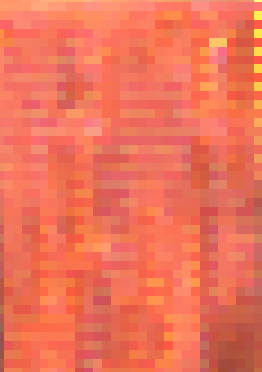
\includegraphics[scale=.5]{../enunciado/images_files/cualitativo/farm_closest.png}
		\vspace{2pt}
		\par
		\footnotesize\textit{Pared de un granero iluminado por el atardecer, algoritmo: Closest Neighbor.}
	\end{center}


	\begin{center}
		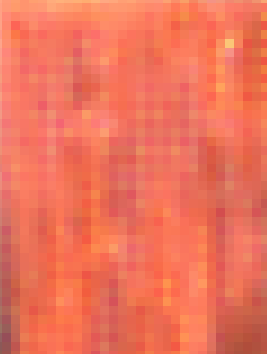
\includegraphics[scale=.5]{../enunciado/images_files/cualitativo/farm_bilinear.png}
		\vspace{2pt}
		\par
		\footnotesize\textit{Pared de un granero iluminado por el atardecer, algoritmo: Bilinear Interpolation.}
	\end{center}


	\begin{center}
		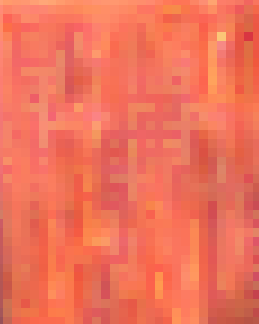
\includegraphics[scale=.5]{../enunciado/images_files/cualitativo/farm_directional.png}
		\vspace{2pt}
		\par
		\footnotesize\textit{Pared de un granero iluminado por el atardecer, algoritmo: Directional Interpolation.}
	\end{center}


	\begin{center}
		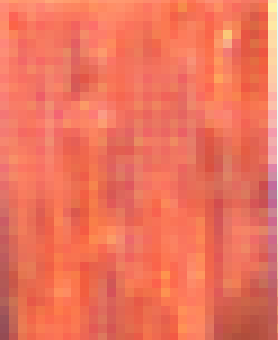
\includegraphics[scale=.5]{../enunciado/images_files/cualitativo/farm_malvar.png}
		\vspace{2pt}
		\par
		\footnotesize\textit{Pared de un granero iluminado por el atardecer, algoritmo: Malvar He Cutler.}
	\end{center}

El algoritmo de vecinos mas cercanos y el de interpolación directional poseen los \textit{artifacts} más notorios. En el primero volvemos a ver la creación de bloques similares a ladrillos en una pared y en el segundo la aparición de laberintos en la imágen.

Consideramos que el algoritmo bilinear devuelve una mejor solución que \textit{Malvar He Cutler} considerando cómo manejan la anomalía de la esquina superior derecha (punto blanco). Dado que el segundo utiliza una vecindad extendida para definir el valor de cada píxel, si se encuentran detalles en la imagen que son resonantes (como un punto de otro color) el algoritmo los propaga de manera más notoria que el bilinear.

Proseguimos con un extracto de la imagen siete: una isla con palmeras.

%.---------------------

	\begin{center}
		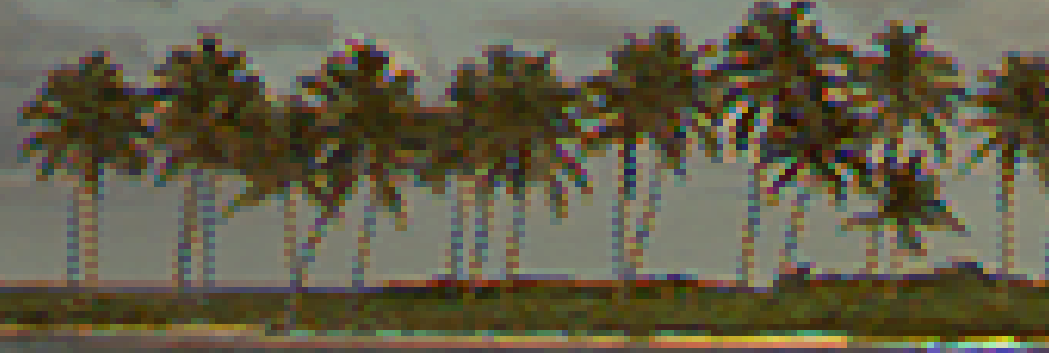
\includegraphics[scale=.5]{../enunciado/images_files/cualitativo/palms_closest.png}
		\vspace{2pt}
		\par
		\footnotesize\textit{Palmeras en el horizonte, algoritmo: Closest Neighbor.}
	\end{center}


	\begin{center}
		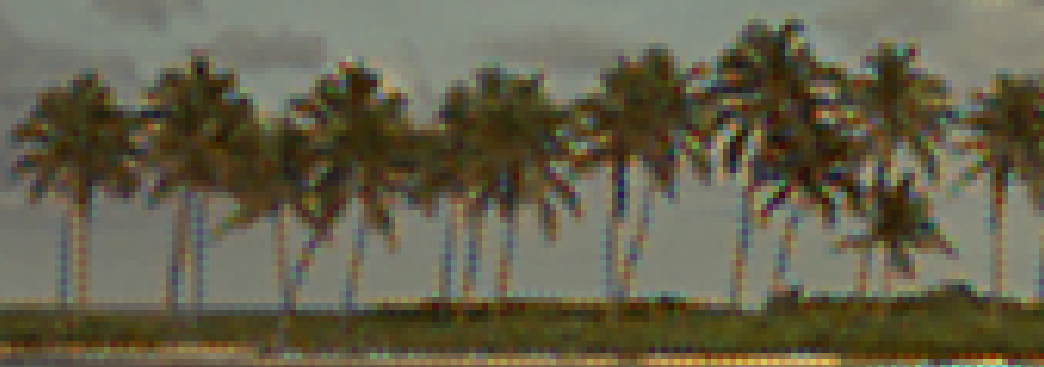
\includegraphics[scale=.5]{../enunciado/images_files/cualitativo/palms_bilinear.png}
		\vspace{2pt}
		\par
		\footnotesize\textit{Palmeras en el horizonte, algoritmo: Bilinear Interpolation.}
	\end{center}


	\begin{center}
		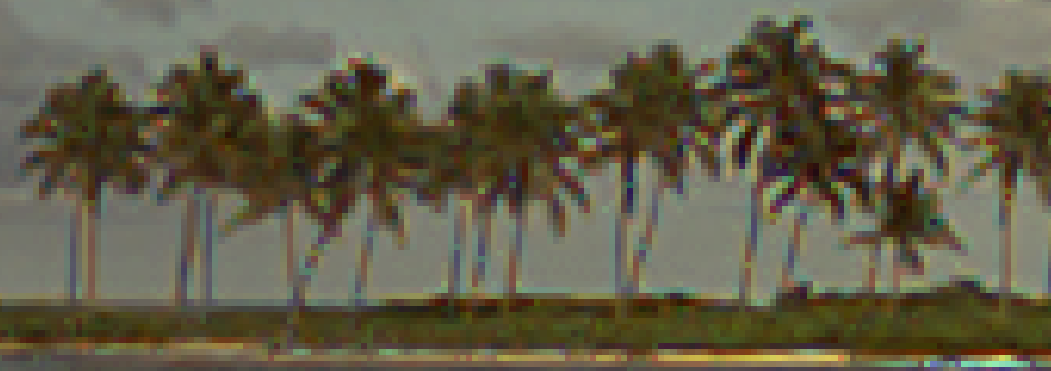
\includegraphics[scale=.5]{../enunciado/images_files/cualitativo/palms_directional.png}
		\vspace{2pt}
		\par
		\footnotesize\textit{Palmeras en el horizonte, algoritmo: Directional Interpolation.}
	\end{center}


	\begin{center}
		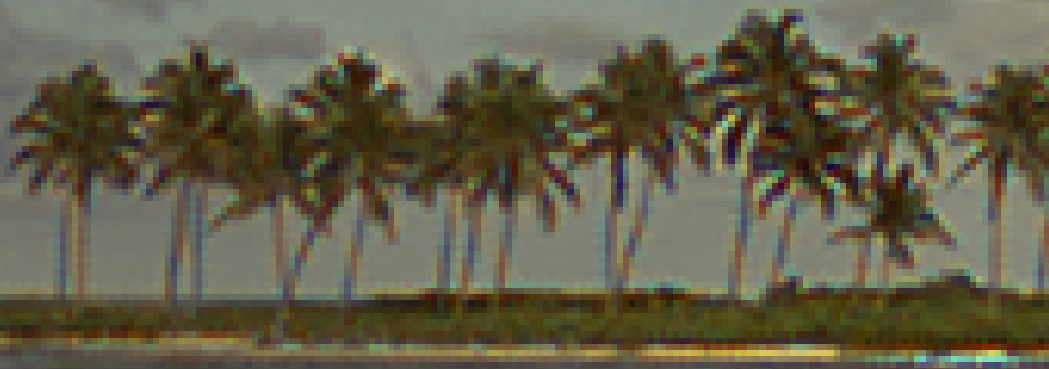
\includegraphics[scale=.5]{../enunciado/images_files/cualitativo/palms_malvar.png}
		\vspace{2pt}
		\par
		\footnotesize\textit{Palmeras en el horizonte, algoritmo: Malvar He Cutler.}
	\end{center}

%.---------------------

	\begin{center}
		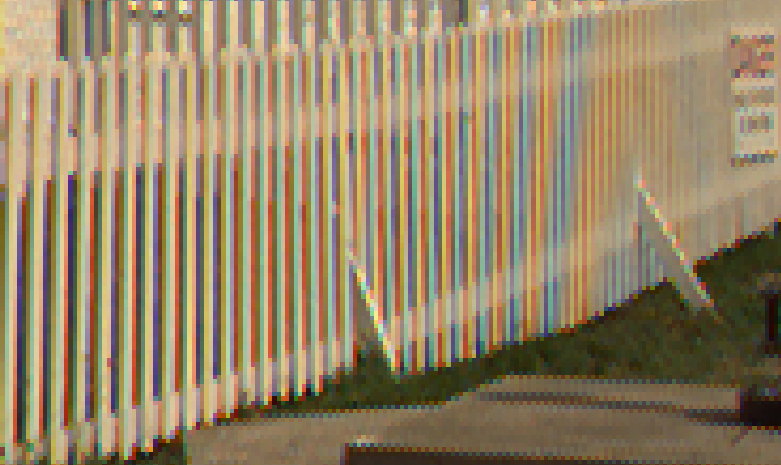
\includegraphics[scale=.5]{../enunciado/images_files/cualitativo/pharo_rails_closest.png}
		\vspace{2pt}
		\par
		\footnotesize\textit{Rejas blancas, algoritmo: Closest Neighbor.}
	\end{center}


	\begin{center}
		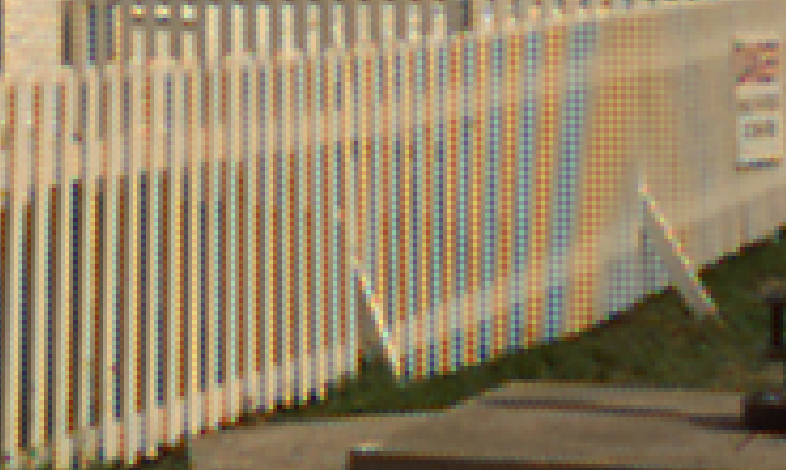
\includegraphics[scale=.5]{../enunciado/images_files/cualitativo/pharo_rails_bilinear.png}
		\vspace{2pt}
		\par
		\footnotesize\textit{Rejas blancas, algoritmo: Bilinear Interpolation.}
	\end{center}


	\begin{center}
		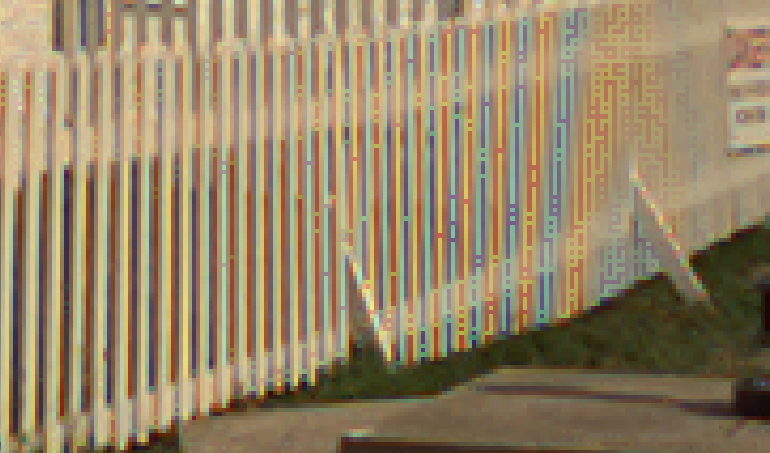
\includegraphics[scale=.5]{../enunciado/images_files/cualitativo/pharo_rails_directional.png}
		\vspace{2pt}
		\par
		\footnotesize\textit{Rejas blancas, algoritmo: Directional Interpolation.}
	\end{center}


	\begin{center}
		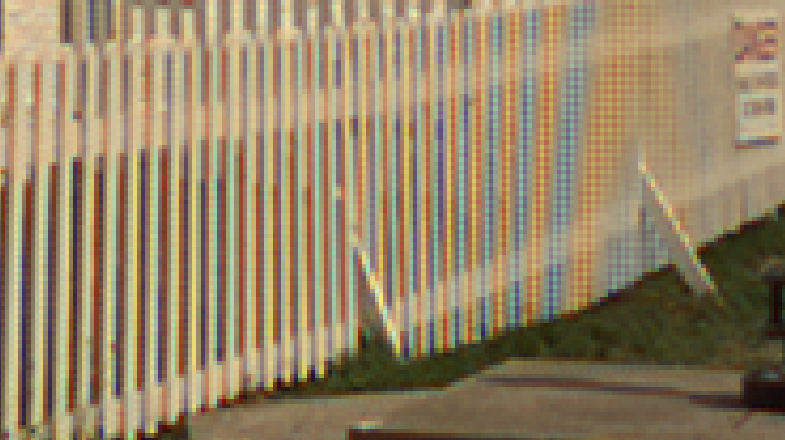
\includegraphics[scale=.5]{../enunciado/images_files/cualitativo/pharo_rails_malvar.png}
		\vspace{2pt}
		\par
		\footnotesize\textit{Rejas blancas, algoritmo: Malvar He Cutler.}
	\end{center}

%.---------------------

	\begin{center}
		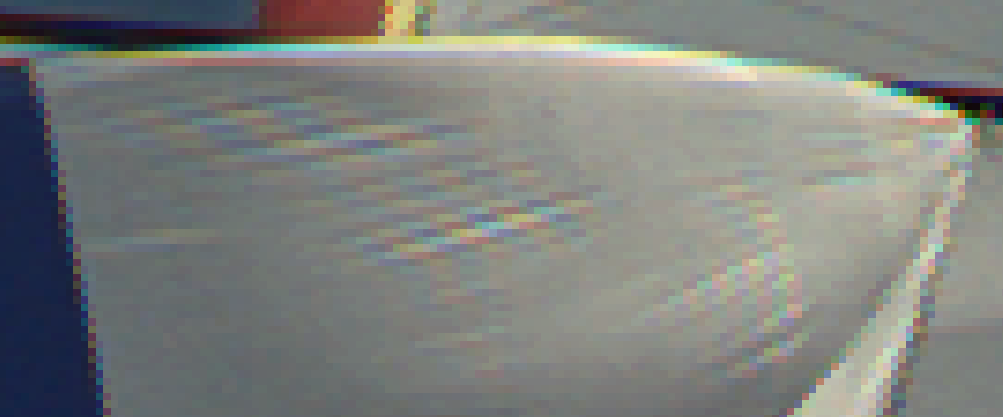
\includegraphics[scale=.5]{../enunciado/images_files/cualitativo/sailing_boat_closest.png}
		\vspace{2pt}
		\par
		\footnotesize\textit{Vela de un velero, algoritmo: Closest Neighbor.}
	\end{center}


	\begin{center}
		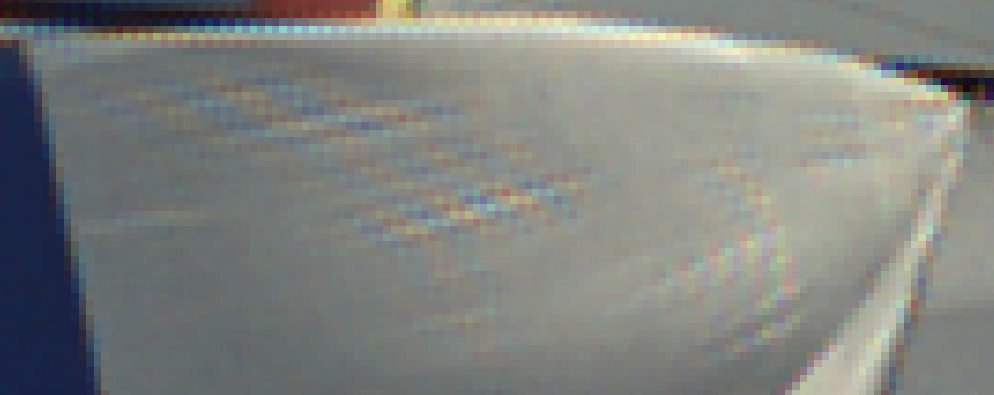
\includegraphics[scale=.5]{../enunciado/images_files/cualitativo/sailing_boat_bilinear.png}
		\vspace{2pt}
		\par
		\footnotesize\textit{Vela de un velero, algoritmo: Bilinear Interpolation.}
	\end{center}


	\begin{center}
		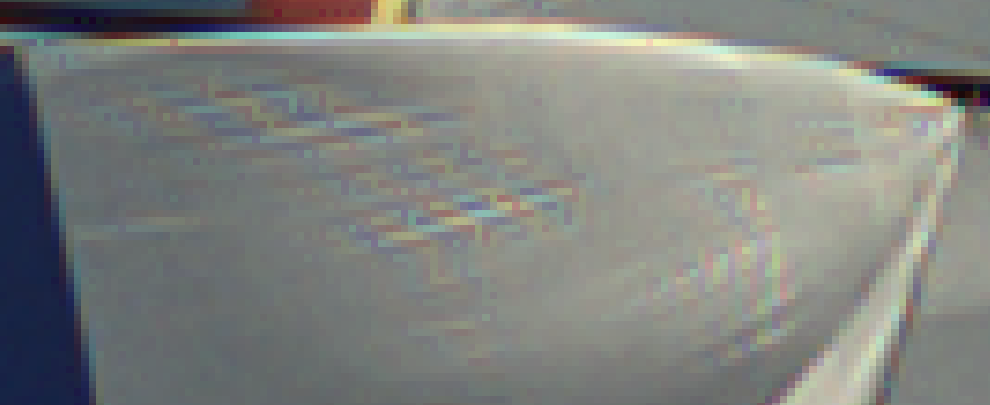
\includegraphics[scale=.5]{../enunciado/images_files/cualitativo/sailing_boat_directional.png}
		\vspace{2pt}
		\par
		\footnotesize\textit{Vela de un velero, algoritmo: Directional Interpolation.}
	\end{center}


	\begin{center}
		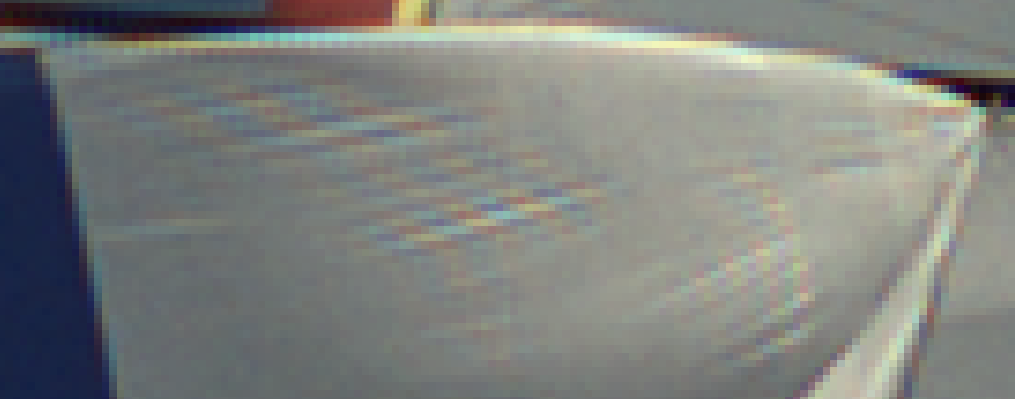
\includegraphics[scale=.5]{../enunciado/images_files/cualitativo/sailing_boat_malvar.png}
		\vspace{2pt}
		\par
		\footnotesize\textit{Vela de un velero, algoritmo: Malvar He Cutler.}
	\end{center}


\section{Conclusión}

Lo interesante a destacar es, que hilando fino, podemos ver que ninguna de las imágenes son iguales. La digitalización de las imágenes nos otorga una mirada sesgada e irreal de la realidad (considerando ``realidad'' como lo que nuestros ojos pueden interpretar).

\section{Bibliografía y referencias} %arreglar cuando se termine 

\begin{itemize}
	\item \textbf{STL de C++}: \url{http://en.cppreference.com}.
%	\par Para la función \texttt{rand()}, \url{http://en.cppreference.com/w/cpp/numeric/random/rand}.
%	\par Para la función \texttt{sort()}, \url{http://en.cppreference.com/w/cpp/algorithm/sort}.
%	\item Distribución de \texttt{rand()}?, \url{http://eternallyconfuzzled.com/arts/jsw\_art\_r and.aspx}
%	\item \textbf{Métodos Numéricos:}
%		\par Método de la potencia: Richard BURDEN, Numerical Analysis 9th Ed. Chapter 9 Section 3, p. 576
%		\par \textit{Papers} del TP.
%	\item \textbf{Contador de clocks}: \url{http://www.mcs.anl.gov/\~kazutomo/rdtsc.html}
http://www.cambridgeincolour.com/tutorials/camera-sensors.htm
http://ins.sjtu.edu.cn/people/mtang/textbook.pdf
\end{itemize}


\end{document}
